\section{Detailed Process}

In this section each phase of the proposed approach is detailed using the running example introduced in the previous section.

\subsubsection{Defiant component identification}

% First step: Modelling normal scenarios 
Initially, we use scenarios to model the core functional requirements for the self-adaptive system and the local requirements for each component. Scenarios formalise both exceptional and normal conditions of the system, which have been widely used for modelling {\it what-if} situations~\cite{Uchitel2003}. It assumes the use of off-the-shelf software components, with predefined requirements and specifications. 

Figure~\ref{fig:drone_msc} shows part of hMSC specification for the payload organ delivery scenario discussed in Section 1. Each box in the hMSC corresponds to a basic message sequence chart (bMSC), exchanging messages between different entities, whilst the bMSC are put together through control flows (branches and loops). Figure~\ref{fig:drone_bmsc} depicts the referred bMSCs for part of the drone payload delivery example.

\begin{figure}
    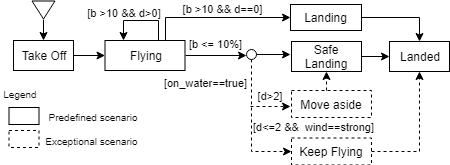
\includegraphics[width=\columnwidth]{figures/new_drone_msc.png}
    \caption{hMSCs for the drone scenario}
    \label{fig:drone_msc}
    \vspace*{-0.25cm}
\end{figure}

\begin{figure}
    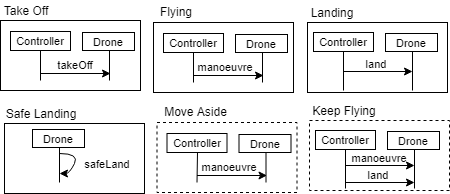
\includegraphics[width=\columnwidth]{figures/new_drone_bmsc.png}
    \caption{bMSCs for the drone delivery scenario}
    \label{fig:drone_bmsc}
    \vspace*{-0.5cm}
\end{figure}

In Figure~\ref{fig:drone_msc}, the predefined scenarios are represented by a full rectangle and are part of the normal specification of a drone, while the exceptions are represented by dashed rectangles. As shown in Figure~\ref{fig:drone_msc}, through a controller the pilot can control the drone to take off, and can manoeuvre the drone when the battery is above a certain threshold $\theta = 10\%$, while it has not reached the destination. When the pilot sends a landing command to the drone, this is acknowledged when the drone lands in the ground.  During a flight, a drone periodically checks the status of its internal devices such as battery level and distance from the destination, represented by \textit{b} and \textit{d}, respectively, in the guard conditions over the transitions. In the example, if the battery level is above the expected threshold and the drone is not yet in its destination, the drone keeps flying. If the drone reaches its destination, it performs a landing action. If the battery is below the expected threshold, the drone performs a safe landing in accordance to its predefined specification. 

% Second step: extend the MSC with exception scenarios
The second step consists of extending the initial scenario specification with the identified exceptional scenarios and context variables. Here we augment the MSC specification with an interception point, that represents the moment on which a condition is analysed in order to decide whether the original expected scenario is executed or an introduced exceptional scenario has to take place instead. 

The exceptional conditions added in the interception point state that if the distance to the expected destination is less than 2km, the drone is flying over the river (condition \textit{on\_water==true}), and the wind is strong (condition \textit{wind==strong}), then the pilot can keep the drone flying even in a low-level battery situation and then land, thus being able to complete its overall goal (delivering the medical payload) successfully. Nonetheless, if the battery is low, the drone is above water, but the drone is more than 2km away or the wind is not strong, then the action is to move the drone aside in order to land it on the ground.

% Paolo: Fig 2 needs update
% "[d > 2]" => "[d > 2 || wind!=strong]"

% Third step: generate the parameterized LTS
Subsequently, the complete MSC scenario specification is automatically transformed to a parameterized Labelled Transition System (LTS), which contains in the scenario transition conditions as guards in the corresponding state transitions that represent the scenario change. The reason for converting scenarios into LTS formally is to facilitate the correctness checks of the model before and after the adaptation. %The scenarios representing the system (with the off-the-shelf components) are transformed into LTS behaviour models, and requirements are transformed into properties. 

The MSC-to-LTS generation algorithm is an adaptation of the one proposed in ~\cite{Rodrigues:2005}, with the introduction of the scenario transition guards in the resulting LTS. Figure~\cite{fig:pLTS} depicts the parameterized LTS generated for the drone example of Figure 1. 

\begin{figure*}\centering
 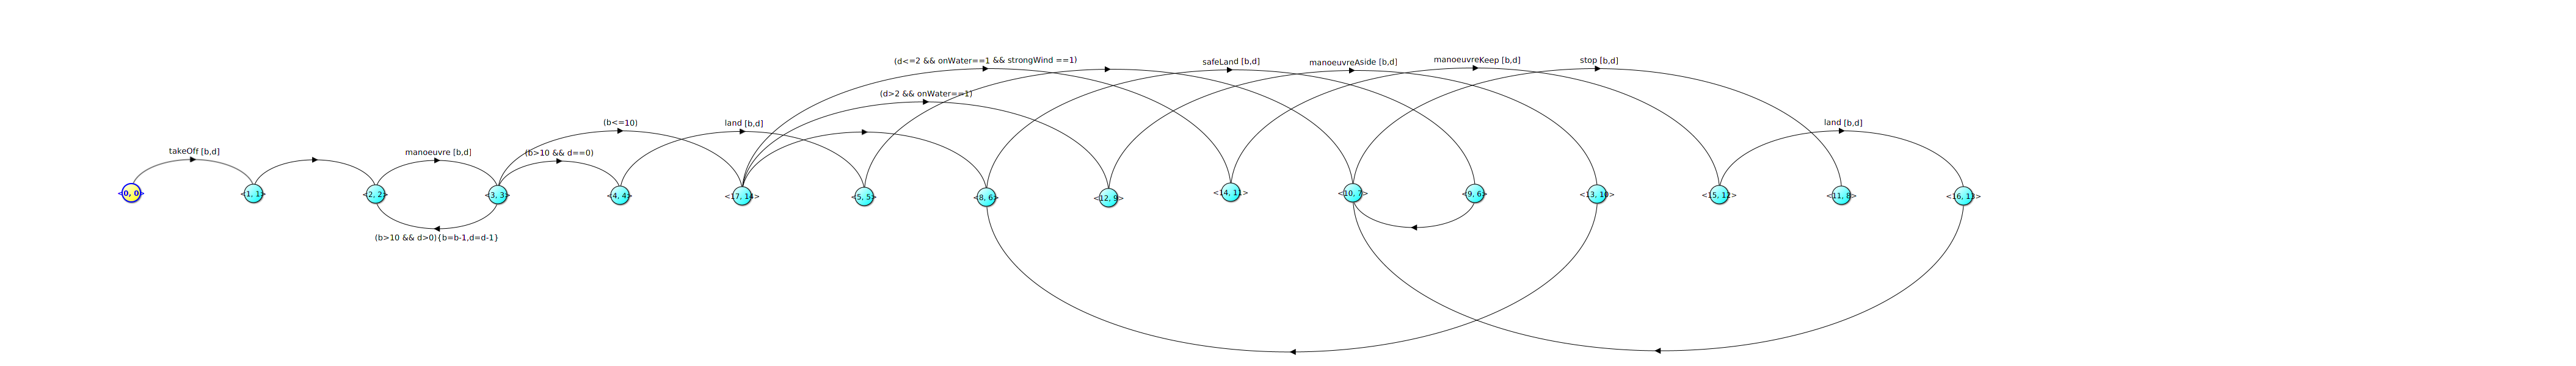
\includegraphics[width=\textwidth]{figures/3-parameterized-LTS.png}
    \caption{Parameterised LTS illustrates the behaviours when the contextual variables are parameters bound to user specified constants. }
    \label{fig:pLTS}
    \vspace*{-0.25cm}
\end{figure*}

%Given the similarities between exceptional and what-if conditions, the approach uses existing formal method techniques, like feedback-driven implied scenario resolutions~\cite{uchitel:2013}, to verify scenarios represented as message sequence charts (MSC) translated into labelled transition systems (LTS), with respect to safety and liveness properties. 
%\textbf{Note: we need a justification here!}

%Fourth step: generation of final LTS 
After that, the user can set the values of the context variables and instanciate a context-specific LTS.

\begin{figure*}\centering
 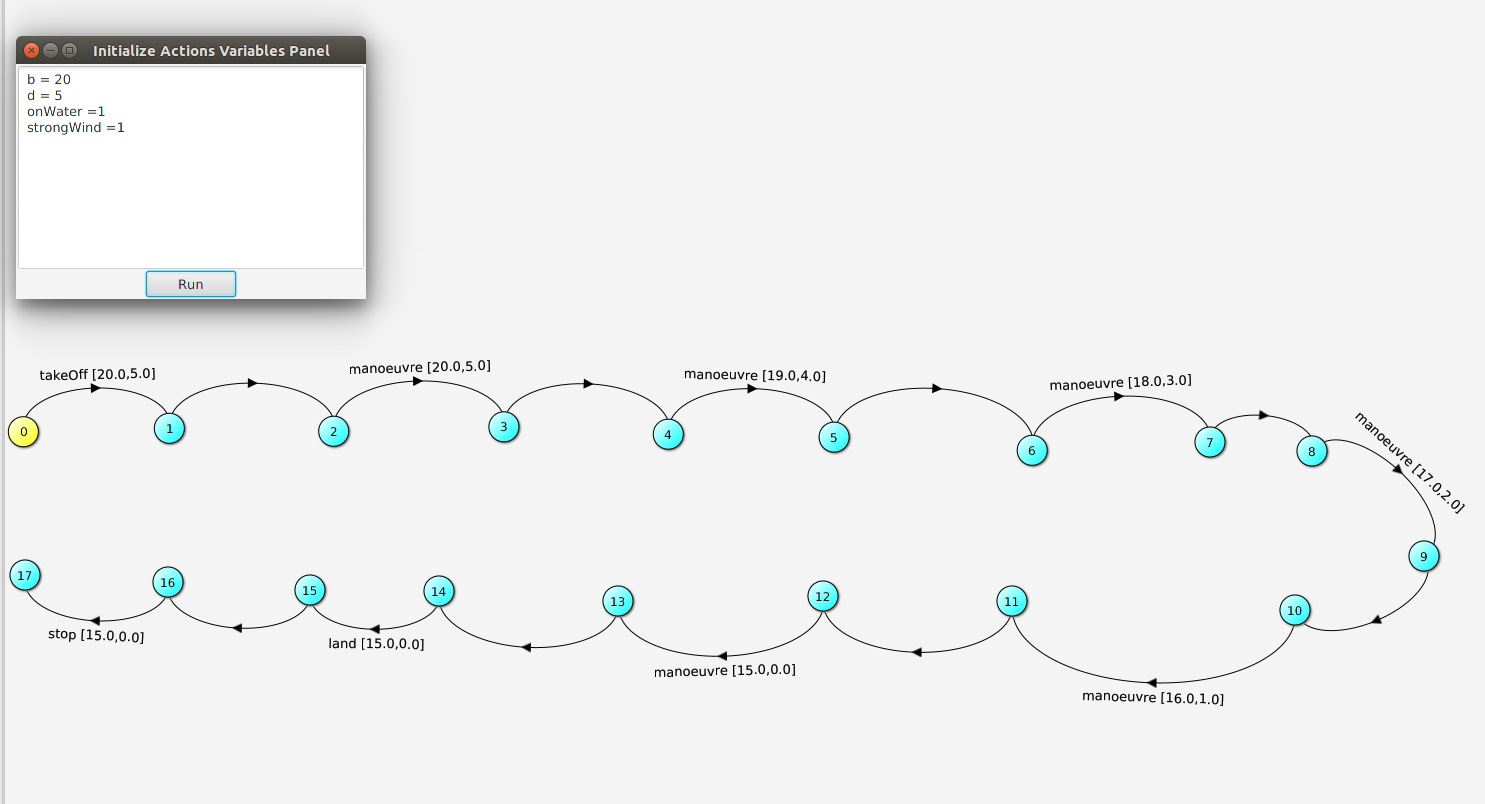
\includegraphics[width=0.8\textwidth]{figures/4-Land-final-LTS.png}
    \caption{LTS of Landing: the partial behaviour of landing bMSC, where the unnamed transitions are the transitions between different bMSCs. Though an $\epsilon$-reduction, these transitions will be removed.}
    \label{fig:landing}
    \vspace*{-0.25cm}
\end{figure*}

%Fifth step: checking local and global requirements
That LTS can be exported to LTSA in order to check both local and global requirement specified in terms of properties. If the generated behaviour satisfies local requirements but does not satisfy the global ones, then a defiant behaviour is identified and has to addressed, otherwise the component can be used as it is in the new system of system.
The verification of the satisfaction arguments of global requirements and local requirements provides designer a formal basis to tell whether or not defiant behaviour exists in the components, and whether or not addressing the defiant behaviours (i.e., an off-the-shelf component cannot satisfy the global requirements out of the box). 

If the identified defiant component can be reconfigured (for instance, via source code alteration or parameterization), then a component reconfiguration occurs. This is out of scope of this research. After that, the new component behaviour is verified again in order to check whether it satisfies the local and global requirements. 

A model checker is applied to verify whether the off-the-shelf component can also satisfy  global requirements of the system-of-system, for which not necessarily it was designed. In the case when the component satisfies the requirements, it can be used as-is in the system-of-system. However, when the component cannot be changed (i.e., the case of a defiant component), a wrapper is specified in order to weave exceptional conditions into the component specification in LTS, and it is verified by the LTSA model checker against the properties.  The adaptation is considered {\it cautious} only when {\bf all} the properties (local and global) are satisfied by the component within the system-of-system context. The verification step is considered successful, that is, the defiant behaviours can be addressed by design-time simulation and verifications. 

\subsubsection{Wrapper Design and Implementation}

In the first step, contextual variables for analysing the global requirements are elicited such as battery levels, distance to destination, drone is over the water or not, and whether or not the wind is favorable, etc.  These variables may not be available or used for analysing the local requirements of the component. Nonetheless, from a bigger picture, usually they are critical to tell the satisfaction of the global requirements. 

The second step aims at analysing situations when the satisfaction of local requirements denies the satisfaction of global requirements in order to identify the exceptional conditions. The what-if situations marks exceptional conditions on an extension of the scenario models, which will also be transformed into safety properties in LTS.  E.g., battery level is lower than 10\%, distance to destination is smaller than 2km, the drone is over the water, and the wind is favourable to cover the remaining distance with fewer power. The combination of these conditions would trigger a situation that it is in fact possible to satisfy the global requirements by the drone, only if some of its existing safety assumption is updated. In the opposite case, the failed checks are used to identify how to deal with exceptional conditions. %From the counter examples provided by the model checker (i.e., sequences of actions that lead to failures), software designers can inspect which of the actions can be avoided by negating the conditions that trigger these action in the behavioural model. These triggered conditions are combined to form exceptional conditions. The negation of an exceptional condition is considered as a normal condition.

In the next step, the exceptions can be addressed by Planning adaptation actions in the component. Using the existing functionalities such as maneuveuring, while disabling certain functionaties such as safe landing, it is possible to switch to a different solution through adaptation. Such adaptions are modelled as advices such as before / around of existing functionalities/actions in the adapted component.

\item {\bf Simulating circumventing behaviours.} Under exceptional conditions the alternative adaptation actions need to be called, however, the existing component is not designed to be adaptable. In this step we uses aspect-oriented mechanisms to weave the changes into the system behaviours and pass the modified behavioural model back to the verification step. Note that this step is still performed at the design time, therefore we cannot call it ``execution", but it is corresponding to the execution step of the MAPE self-adaptive system at the runtime.

After the wrapper has been implemented, the last step consists on deploying it on the system so it can adapt at runtime the behaviour of the defiant components.

\subsubsection{Runtime Cautious Adaptation}

Here comes the text... 